\documentclass[12pt]{article}
\raggedbottom
% ==================================================
% CONFIGURACIÓN DE PÁGINA
% ==================================================
\usepackage[
a4paper,
top=3cm,
bottom=3cm,
left=2cm,
right=2cm
]{geometry}

% ==================================================
% IDIOMA Y CODIFICACIÓN
% ==================================================
\usepackage[T1]{fontenc}
\usepackage[utf8]{inputenc}
\usepackage[spanish, es-tabla]{babel}

% ==================================================
% MATEMÁTICAS
% ==================================================
\usepackage{amsmath,amssymb,amsfonts}

% ==================================================
% IMÁGENES Y TABLAS
% ==================================================
\usepackage{graphicx}
\usepackage{tabularx}
\usepackage{array}
\usepackage{booktabs}
\usepackage{float}
\usepackage{caption}

\newcolumntype{Y}{>{\centering\arraybackslash}X}

% ==================================================
% FORMATO DE TEXTO
% ==================================================
\usepackage{titlesec}

\setlength{\parskip}{0.5em}
\setlength{\textfloatsep}{5pt}
\setlength{\intextsep}{10pt}

\parindent=0cm

% Numeración y profundidad
\setcounter{secnumdepth}{5}
\setcounter{tocdepth}{5}

% Formato de párrafos
\titleformat{\paragraph}[block]
{\normalfont\normalsize\bfseries}
{\theparagraph}
{1em}
{}

\titlespacing*{\paragraph}
{0pt}
{1ex plus 0.5ex minus .2ex}
{1ex}

% ==================================================
% ENCABEZADOS Y PIE DE PÁGINA
% ==================================================
\usepackage{fancyhdr}

\pagestyle{fancy}
\fancyhf{}

% Logo izquierdo
\fancyhead[L]{
	
\includegraphics[height=1.5cm]{../figuras/Imagenes/Logo_1.png}
}

% Texto derecho
\fancyhead[R]{
	\parbox{4cm}{
		\centering
		\textbf{Instrumentación\\Geotécnica}
	}
}

% Pie de página
\fancyfoot[C]{Página \thepage}

% Líneas
\renewcommand{\headrulewidth}{0.4pt}
\renewcommand{\footrulewidth}{0.4pt}

% Ajustes encabezado
\setlength{\headheight}{45pt}
\setlength{\headsep}{12pt}

% ==================================================
% HIPERVÍNCULOS
% ==================================================
\usepackage[
unicode,
colorlinks=true,
linkcolor=black,
urlcolor=blue,
citecolor=black
]{hyperref}

% ==================================================
% BIBLIOGRAFÍA
% ==================================================
\usepackage{csquotes}

\usepackage[
backend=biber,
style=apa,
sortcites,
url=true
]{biblatex}

\addbibresource{biblio.bib}

% ==================================================
% NOMBRES EN ESPAÑOL
% ==================================================
\addto\captionsspanish{
	\renewcommand{\contentsname}{Tabla de contenido}
	\renewcommand{\listfigurename}{Lista de figuras}
	\renewcommand{\listtablename}{Lista de tablas}
}

% ==================================================
% DOCUMENTO
% ==================================================

% ===== DOCUMENTO =====
\begin{document}
	
	
	\begin{titlepage}
		\centering
		% Logo de la universidad (ajusta el nombre del archivo)
		
\includegraphics[width=0.2\textwidth]{../figuras/Logo_1.png}\par\vspace{1cm}
		
		
		% Título del trabajo
            {\Large \textbf{ESTUDIO DE AMENAZA SÍSMICA PARA LA CIUDAD DE NEIVA}}\par
		\vspace{2.5cm}
		
		% Autores
		{\Large \textbf{ELABORADO POR:}\\
			ANDRÉS STIVEN JARAMILLO CATAÑO\\
			EMMEL ESCOVITHCH RIAÑO\\
                  LAURY YOCELY PEREA MENA\par}
		\vspace{2.5cm}
		
		% Autores
		{\Large \textbf{DOCENTE:}\\
			ANDRES FELIPE SERNA VAZQUEZ\par}
		\vspace{2.5cm}
		
		% Facultad y departamento
		{\large \textbf{
				Universidad Nacional de Colombia\\
				Facultad de Ingeniería\\
				Departamento de Ingeniería Civil}}
		
		\vfill
		% Fecha
		\textbf{{\large OCTUBRE 2026}}
	\end{titlepage}



	
	\pagestyle{fancy}
	
	% Limpiar encabezado y pie
	\fancyhf{}
	
	% ===== ENCABEZADO =====
	\fancyhf{} % limpia todo
	
	\fancyhead[L]{\raisebox{5pt}{
\includegraphics[height=2cm]{../figuras/Logo_encabezado.png}}}
	
	\fancyhead[R]{%
		\raisebox{10pt}{
			\parbox{4cm}{\centering
				\large\textbf{Instrumentación Geotécnica}}
		}
	}
	
	
	
	% ===== PIE DE PÁGINA =====
	\fancyfoot[C]{Página \thepage}
	
	% Líneas superior e inferior
	\renewcommand{\headrulewidth}{0.4pt}
	\renewcommand{\footrulewidth}{0.4pt}
	
	% Ajusta la altura del encabezado
	\setlength{\headheight}{45pt}
	
	\setlength{\headsep}{30pt}      
	
	
	
\tableofcontents
\listoffigures
	

\newpage

% ============================================================
\section{Introducción y objetivo}

Este informe documenta el avance del trabajo de amenaza sísmica para la ciudad de
Neiva (Huila). El objetivo del trabajo es construir un catálogo sísmico depurado
para Neiva, a partir de las fuentes del Servicio Geológico Colombiano (SGC) y del
United States Geological Survey (USGS), dentro de radios de 50~km y 260~km medidos
desde un punto de referencia en el centro de la ciudad. Este catálogo es el insumo
principal para el posterior análisis de amenaza sísmica, la construcción del
espectro en roca según la NSR-10 y la selección de acelerogramas compatibles.

Por el momento, este documento recoge únicamente la etapa de recopilación y
organización de la información sísmica: el punto de referencia adoptado, las
fuentes y parámetros de búsqueda utilizados, y las decisiones metodológicas
tomadas hasta la fecha. Las etapas de homogenización de magnitudes, depuración
y análisis de amenaza se incorporarán en versiones posteriores de este informe.

% ============================================================
\section{Zona de estudio y punto de referencia}

Como punto de referencia para la búsqueda del catálogo sísmico se adoptó el
\textbf{Parque Central Santander}, en el centro cívico e institucional de Neiva,
con coordenadas:

\begin{center}
    Latitud: $2.9262767$\textdegree \qquad Longitud: $-75.2892111$\textdegree
\end{center}

A partir de este punto se definieron dos radios de búsqueda:

\begin{itemize}
    \item \textbf{50 km}: catálogo cercano, relevante para la amenaza sísmica
          local y la sismicidad asociada a fuentes próximas a la ciudad.
    \item \textbf{260 km}: catálogo regional, que permite capturar fuentes
          sismogénicas distantes (por ejemplo, la subducción del Pacífico y
          sistemas de falla regionales) que también pueden contribuir a la
          amenaza sísmica de Neiva. Este radio se adoptó, en lugar de uno de
          200~km, para garantizar que la sismicidad asociada al municipio de
          San José del Palmar (Chocó) quede dentro de la zona de estudio: sus
          epicentros se encuentran entre 232 y 260~km del punto de referencia.
    \end{itemize}

La Figura~\ref{fig:mapa_zona} muestra el punto de referencia y ambos radios
de búsqueda sobre una imagen satelital de la región. Neiva se encuentra en
el valle interandino del Alto Magdalena, entre las cordilleras Central y
Oriental; el radio de 260~km alcanza ciudades como Cali, Ibagué, Popayán y
Bogotá, y se extiende hasta la zona de subducción del Pacífico.

\begin{figure}[htbp]
    \centering
    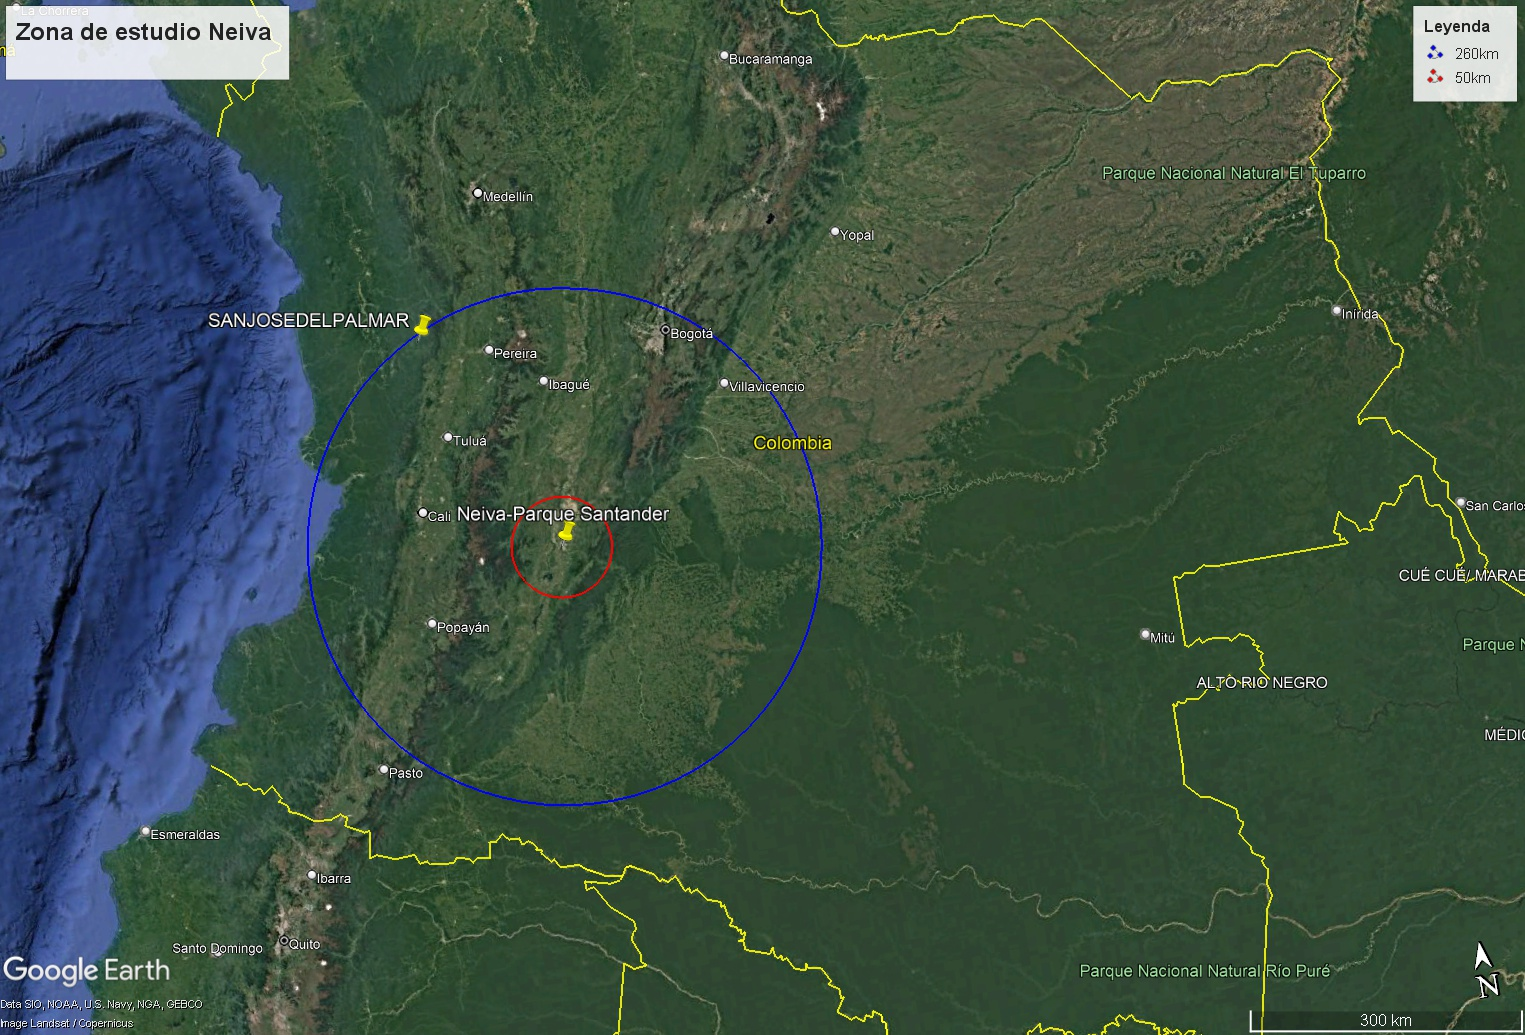
\includegraphics[width=0.8\textwidth]{../figuras/zonadeestudioradio260.jpg}
    \caption{Zona de estudio: punto de referencia en Neiva (Parque Central
    Santander), radios de búsqueda de 50 y 260~km y ubicación de San José del
    Palmar. Imagen satelital: Google Earth.}
    \label{fig:mapa_zona}
\end{figure}

Como primer acercamiento a la sismicidad de la zona, la Figura~\ref{fig:mapa_epicentros}
muestra los epicentros del catálogo consolidado (SGC y USGS) dentro de
260~km, coloreados por magnitud y diferenciados por fuente (círculos para
el SGC, triángulos para el USGS). Se aprecia una alineación de sismicidad
de suroeste a noreste, consistente con el sistema de fallas regional de la
zona (Algeciras--Suaza), además de un cúmulo de sismicidad más profunda
hacia el occidente, asociado a la zona de subducción. Los eventos del USGS
se concentran en las magnitudes más altas de cada zona, consistente con lo
discutido en la Sección~\ref{sec:estado}.

\begin{figure}[htbp]
    \centering
    
\includegraphics[width=0.85\textwidth]{../figuras/mapa_zona_estudio.png}
    \caption{Epicentros del catálogo consolidado SGC + USGS dentro de
    260~km alrededor de Neiva, coloreados por magnitud y diferenciados por
    fuente.}
    \label{fig:mapa_epicentros}
\end{figure}

% ============================================================
\section{Catálogo sísmico: fuentes y metodología}

\subsection{Fuentes de datos utilizadas}

Se utilizaron dos fuentes de información sismológica:

\begin{itemize}
    \item \textbf{SGC -- Red Sismológica Nacional de Colombia (RSNC)}: catálogo
          oficial de sismicidad de Colombia, operado por el Servicio Geológico
          Colombiano. Por ser una red local densa, este catálogo captura
          microsismicidad (magnitudes menores a 2) que las redes globales no
          alcanzan a detectar cerca del territorio colombiano.
    \item \textbf{USGS -- ANSS Comprehensive Earthquake Catalog (ComCat)}:
          catálogo global del United States Geological Survey, construido a
          partir de redes sismológicas mundiales. Es comparativamente completo
          para sismos grandes (magnitud $\gtrsim 4$), pero no detecta de forma
          confiable la microsismicidad local.
\end{itemize}

\subsection{Parámetros de búsqueda}

Para las cuatro combinaciones de fuente y radio se utilizó el mismo punto de
referencia, sin límite inferior de magnitud (magnitud mínima $=0$, es decir,
sin filtrar) y considerando el rango histórico completo disponible en cada
fuente, con el fin de conservar el catálogo lo más completo posible. Los
parámetros específicos se resumen en el Cuadro~\ref{tab:parametros}.

\begin{table}[htbp]
    \centering
    \caption{Parámetros de búsqueda utilizados por fuente.}
    \label{tab:parametros}
    \begin{tabular}{lll}
        \toprule
        Parámetro & SGC & USGS \\
        \midrule
        Servicio / endpoint & \texttt{apicatalogador.sgc.gov.co} & \texttt{earthquake.usgs.gov} (FDSN) \\
        Centro de búsqueda & lat/lon del punto de referencia & lat/lon del punto de referencia \\
        Radios & 50 km y 260 km & 50 km y 260 km \\
        Magnitud mínima & sin filtro (0) & 0 \\
        Rango de fechas & histórico completo & 1900-01-01 -- fecha de descarga \\
        Formato de salida & JSON $\rightarrow$ CSV & CSV \\
        \bottomrule
    \end{tabular}
\end{table}

\subsection{Decisiones metodológicas}

Durante la recopilación del catálogo se tomaron las siguientes decisiones,
que se documentan aquí por su relevancia para la trazabilidad del trabajo:

\begin{itemize}
    \item \textbf{Elección del punto de referencia.} Se adoptó el Parque
          Central Santander por ser el centro cívico e institucional de Neiva,
          un punto estable y fácilmente verificable en cartografía, en lugar
          de, por ejemplo, el centroide del área urbana o la ubicación de una
          estación acelerográfica particular.

    \item \textbf{Catálogo completo del SGC, no solo el resultado por defecto
          de la interfaz web.} La herramienta de consulta pública del SGC
          (\url{https://sismo.sgc.gov.co}) internamente restringe o pagina los
          resultados que muestra en pantalla. Se identificó el servicio REST
          que alimenta la página oficial de descarga del catálogo
          (\texttt{https://apicatalogador.sgc.gov.co/api/events/search/}), y se
          consultó de forma paginada (1000 registros por página) hasta reunir
          la totalidad de los eventos reportados dentro de cada radio, en
          lugar de conformarse con un subconjunto parcial.

    \item \textbf{Sin filtro de magnitud mínima.} Siguiendo la regla de
          trabajo acordada de no descartar información sin autorización
          explícita, se dejó la magnitud mínima en 0 en ambas fuentes, de
          modo que el catálogo conserve incluso los sismos de magnitud muy
          baja. La depuración y homogenización de magnitudes se hará en una
          etapa posterior, sin eliminar registros.

    \item \textbf{Corrección de codificación de caracteres.} En la descarga
          automatizada del catálogo del SGC se detectó y corrigió un problema
          de codificación que producía caracteres corruptos en los nombres de
          municipios con tildes o eñes (por ejemplo, ``Caguán'' o
          ``Caquetá''), asegurando que el texto se decodificara correctamente
          como UTF-8.

    \item \textbf{Dos fuentes, no una sola.} Se mantienen ambos catálogos
          (SGC y USGS) por separado en \texttt{datos originales/} en lugar de
          usar solo uno, dado que son complementarios: el SGC aporta
          completitud en magnitudes bajas y el USGS aporta soluciones
          independientes (incluyendo magnitud de momento $M_w$) útiles para
          la homogenización de escalas de magnitud en la siguiente etapa.

    \item \textbf{Fila duplicada por la descarga.} En el catálogo del SGC a
          260~km, el evento SGC2015gaurko apareció dos veces con datos
          idénticos por un solapamiento entre páginas de la descarga; se
          conservó una sola copia. No se eliminó ningún otro registro.
\end{itemize}

% ============================================================
\section{Estado actual del catálogo}
\label{sec:estado}

El Cuadro~\ref{tab:estado} resume el estado actual de los cuatro catálogos
descargados, disponibles en \texttt{datos/datos originales/} del repositorio
del proyecto.

\begin{table}[htbp]
    \centering
    \caption{Estado actual de los catálogos descargados.}
    \label{tab:estado}
    \begin{tabular}{llrrr}
        \toprule
        Fuente & Radio & N.\ de eventos & Magnitud mín. & Magnitud máx. \\
        \midrule
        SGC  & 50 km  & 2\,380  & 0.7    & 5.0 \\
        SGC  & 260 km & 67\,781 & $-0.1$ & 7.4 \\
        USGS & 50 km  & 20      & 3.4    & 5.5 \\
        USGS & 260 km & 823     & 0.0    & 7.4 \\
        \bottomrule
    \end{tabular}
\end{table}

Se observa una diferencia de casi dos órdenes de magnitud entre el número de
eventos del SGC y del USGS para el mismo radio. Esto es un resultado esperado
y no un error: el SGC opera una red local densa que detecta sismicidad de
magnitud muy baja cerca del territorio colombiano, mientras que el catálogo
global del USGS solo es razonablemente completo para magnitudes mayores a,
aproximadamente, 3.5--4.0 en esta región. En el rango de sismos grandes
($M \geq 4$) ambos catálogos reportan cantidades del mismo orden a 260~km (400
eventos en el SGC y 454 en el USGS), lo que es consistente con esta
explicación. Que el USGS reporte algo más se debe, en buena parte, a su
cobertura temporal: su catálogo inicia en 1917, mientras que el del SGC inicia
en 1993 (desde 1993, el USGS reporta 319 eventos con $M \geq 4$).

Los catálogos se descargaron el 21 de septiembre de 2026. Las magnitudes de
cada fuente se presentan en su escala original; aún no se han homogenizado.

% ============================================================
\section{Próximos pasos}

\begin{itemize}
    \item Unificar los cuatro catálogos en una sola tabla, dentro de
          \texttt{datos/datos depurados/}.
    \item Homogenizar los distintos tipos de magnitud reportados (ML, MLr,
          Mw, mb, entre otros) a magnitud de momento $M_w$.
    \item Revisar formatos de fecha, separadores decimales y profundidades
          reportadas.
    \item Identificar sismos duplicados entre fuentes (sin eliminarlos, solo
          señalarlos para revisión).
    \item Construcción del espectro en roca para Neiva según la NSR-10 y
          selección o generación de acelerogramas compatibles.
\end{itemize}

% ============================================================
\section*{Fuentes consultadas}

\begin{itemize}
    \item Servicio Geológico Colombiano, Catálogo de Sismicidad -- Red
          Sismológica Nacional de Colombia.
          \url{https://sismo.sgc.gov.co}
    \item United States Geological Survey, ANSS Comprehensive Earthquake
          Catalog (ComCat) -- FDSN Event Web Service.
          \url{https://earthquake.usgs.gov/fdsnws/event/1/}
    \item NSR-10, Título A y Título H. Sociedad Colombiana de Geotecnia.
\end{itemize}

\end{document}
